\insertbigimage{figures/block_diagram.pdf}{Block diagram of the system}{block_diagram}

\section{System Design Overview}

The system was designed around the RP2040 microcontroller, acting as the central 
processing unit for interfacing with a variety of sensors and control devices. 
The design incorporates the SF-5M sap flow sensor, LT-1T leaf temperature sensor, 
and MT-603 load cell to measure various environmental parameters. Each of these 
sensors uses different communication protocols, requiring careful consideration of 
power requirements, signal integrity, and communication compatibility.

\note{....}
As seen in \cref{block_diagram}, the system consists of 

\subsection{Hardware Design}
Load Cell and ADC Integration: The MT-603 load cell required an ADC (Analog-to-Digital Converter) for signal conversion, as its output is an analog signal representing weight measurements. One of the RP2040's ADC pins was utilized to convert the load cell's voltage output into a digital signal that the microcontroller could process. This ADC integration allowed for precise scaling and calibration of the load cell to achieve accurate data representation.

SDI-12 Sensors and Communication Interface: The SDI-12 protocol was used because it is the standard communication protocol for the environmental sensors (Sap Flow Sensor and
Leaf thermistor) integrated into this system. However, SDI-12 differs from typical UART communication in that its bit values are inverted. To address this, the project leveraged the RP2040's UART capabilities in conjunction with an RS485 transceiver, using only the B line of the differential pair to handle the inverted logic levels. By setting the voltage reference at 2.5V, the design effectively mapped the inverted SDI-12 signals to conventional UART high and low values, allowing reliable sensor communication.

Power Supply and Voltage Regulation: Due to the diversity of communication protocols and components used in the system—such as ADC for the load cell, SDI-12 for sensors, and I2C for the DAC—multiple voltage levels were required on the PCB: 12V, 5V, and 3.3V. Each voltage level was supplied through dedicated regulators to ensure stable power delivery to each module. The careful placement of decoupling capacitors was critical to minimize voltage ripple and noise, ensuring stable operation of the entire system.

Data Logging and Storage: An SD card module was added to the schematic, utilizing the SPI interface as defined in the RP2040 datasheet. This module enabled reliable data storage and allowed easy access to logged data for further analysis.

DAC Integration: The MCP4716 DAC was integrated to provide fine-grained control of the dew point generator. Proper bypass capacitors were placed near the Vdd pin to minimize induced noise and ensure stable operation.

An initial approach to converting a digital signal to an analogue signal was Pulse Width Modulation (PWM). 
However, this method proved unreliable and inaccurate when tested with a Raspberry Pi Pico. As a result, a digital to analogue converter (DAC) was selected instead.

\begin{figure}
    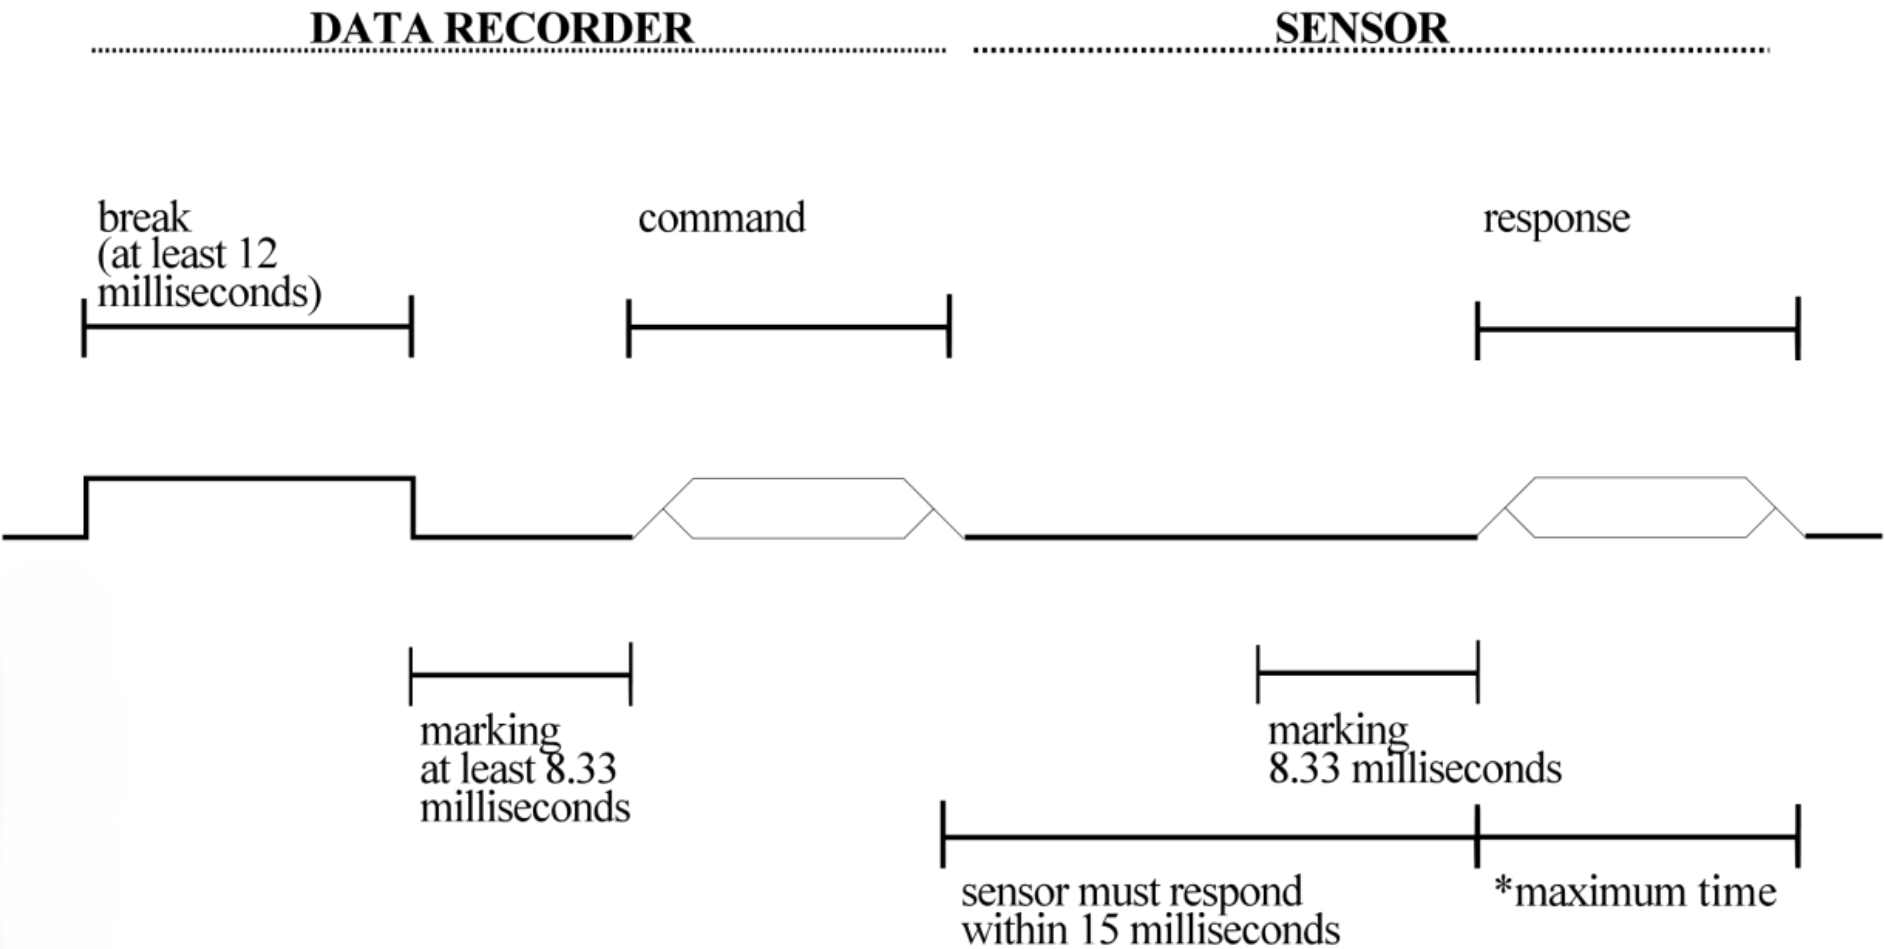
\includegraphics[width=\linewidth]{figures/SDI-12_timing.png}
    \caption{SDI-12 timing from \cite{sdi12_datasheet}}
    \label{sdi12_timing}
\end{figure}

\subsection{Software Design}
Sensor Data Acquisition: Custom drivers were developed for each sensor, adhering to the SDI-12 protocol. Specific issues with the byte framing of the SDI-12 protocol were addressed by using the \code{uart_set_format()} function to configure the communication format correctly, allowing the RP2040 to receive the inverted data without additional circuitry. We used the \code{uart_break()} function to send the break signal, and then used the \code{uart_read_stuff()} function to read the response from the sensor. The response was then parsed to get the data. The timing of the SDI-12 protocol is shown in \cref{sdi12_timing}.

Data Storage: The FatFs API was integrated to enable read/write operations on the SD card, using the SPI protocol. This allowed for structured data logging and easy retrieval of information.

Control Interface: A software interface for controlling the dew point generator was implemented using the I2C protocol to communicate with the DAC. This interface allowed precise voltage adjustments to the generator, with preliminary tests confirming accurate output predictions based on command inputs.

The careful selection of communication interfaces and voltage levels, along with robust software integration, allowed the system to operate seamlessly and efficiently, providing a reliable solution for monitoring and controlling environmental parameters.